
\section{Average number of generations until equilibrium}
There are lots of parameters that may affect the average generations until  equilibrium is reached. We chose to look at the influence of the Happiness Rule(HR) on the average generations. For each HR ranging from 0 to 1 with increment 0.01, we ran 500 simulations and calculated the average, maximum and minimum generations it took to reach equilibrium. The results are shown in figure \ref{fig:avegen}.\\
\\
In figure \ref{fig:avegen}, we observe that the average number of generations (blue graph) is increasing with the Happiness Rule, which is expected since a higher HR requires more neighbours of the same type. We also note that at around a HR of 0.7, the average number of generations becomes more or less constant. That is also expected, because the requirement for the neighbours will be the same. For example, with a happiness of 0.8, a person with 3, 5 or 8 neighbours would require respectively 3, 5 or at least 7 of the same types. This requirement won't change much if a HR of 0.9 is applied. The same argument also explains why the average number of generations is constant at very low HR or for HR with little difference. So it would be sufficient if we ran the simulations with increment for example 0.1.\\
\\
\begin{figure}[h!]
    \centering
    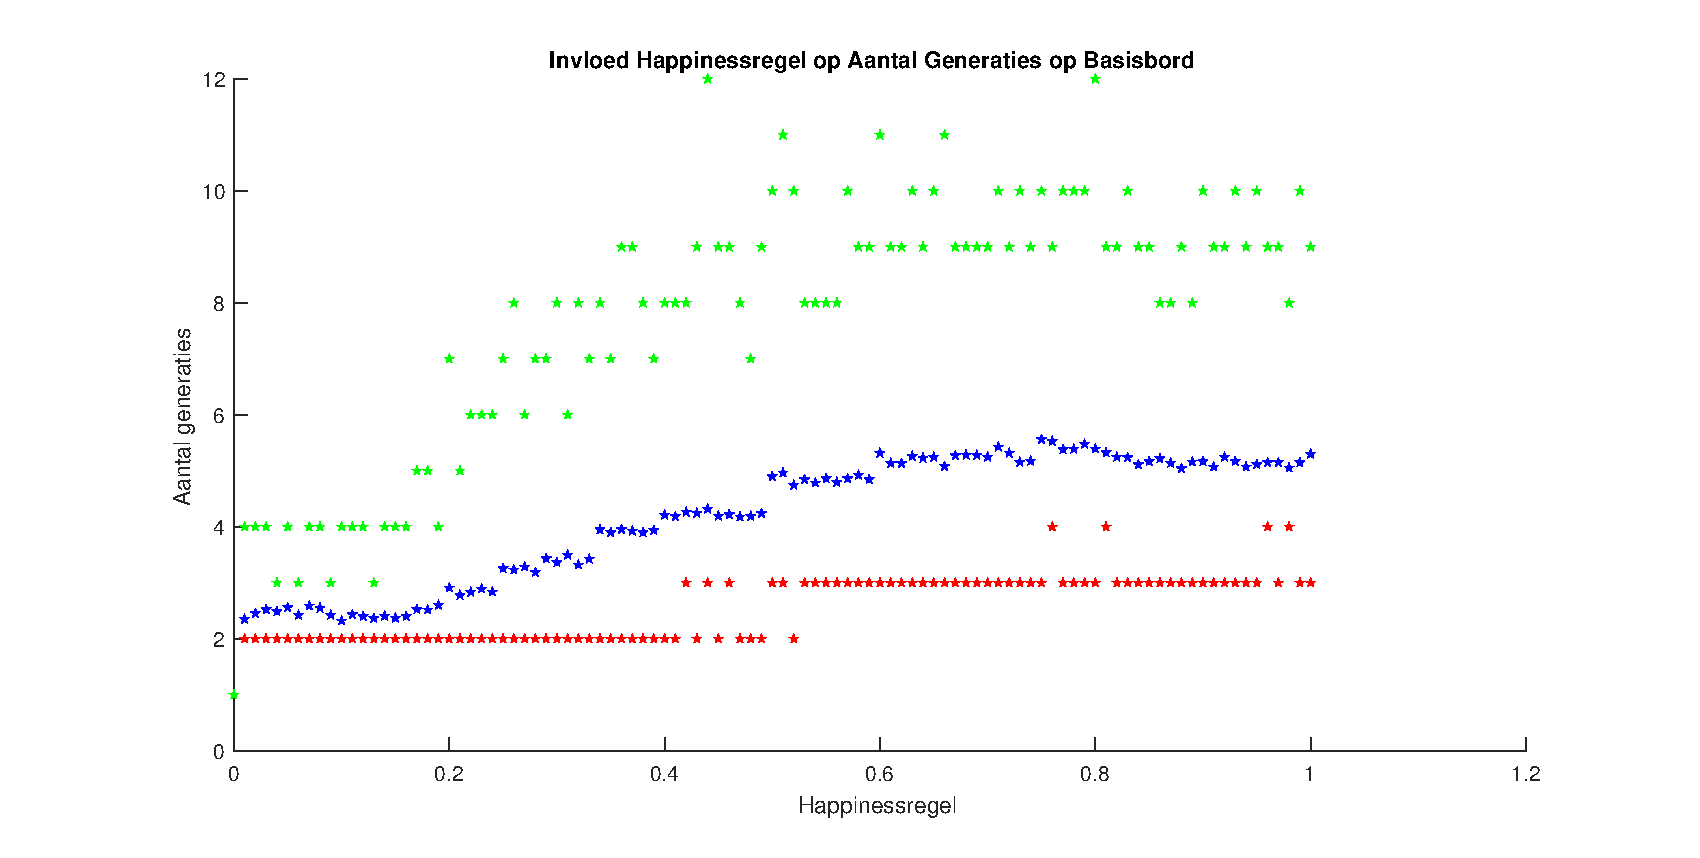
\includegraphics[width=0.9\textwidth]{happinessregel_aantgen_2}
    \caption{Influence of happiness rule on the number of generations until reaching the equilibrium. The green graph shows the maximal generations, the blue graph shows the average generations and the red graph shows the minimal generations}
    \label{fig:avegen}
\end{figure}
\\
It is also interesting to know how the random variable $Y$, which we denote as the number of generations it takes to reach the equilibrium, is distributed. Since $Y$ depends on the position of each individual, whose position also depends on other individuals, the probability distribution of $Y$ might be complicated. Therefore, we approximated the distribution of $Y$ with a histogram (figure \ref{fig:histogram}) of bin size 1, which is reasonable because $Y$ only takes integer values. Also, to look at the influence of the HR on the distribution of $Y$, we made histograms for HR of 1/4, 1/3, 1/2 and 1.  We believe that the histograms are a good model for the distribution for $Y$, since accroding to the law of large numbers, the histogram will converge to the actual distribution since it is obatained after 10000 simulations.\\
\\
 
\begin{figure}[H]
	
    \centering
    \begin{subfigure}{0.4\textwidth}
        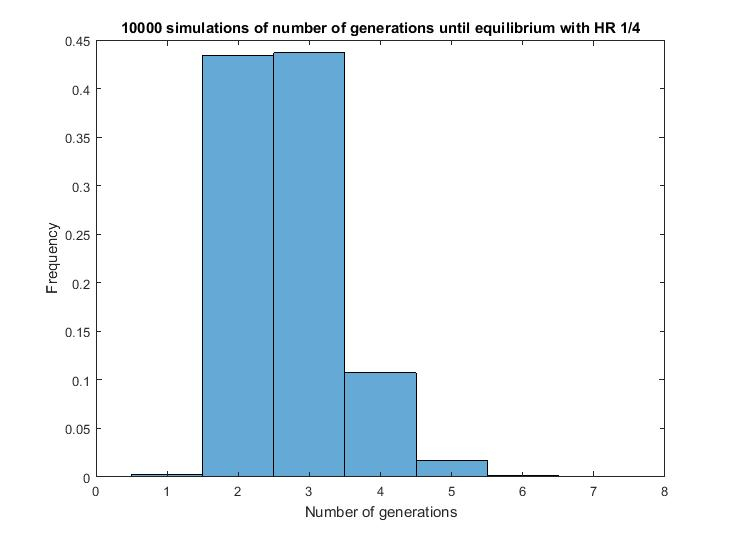
\includegraphics[width=\textwidth]{GenormHistogramAantalgen4}
        \caption{10000 simulations of number of generations until equilibrium with HR 1/4}
        \label{fig:gull}
    \end{subfigure}
    ~ %add desired spacing between images, e. g. ~, \quad, \qquad, \hfill etc. 
      %(or a blank line to force the subfigure onto a new line)
    \begin{subfigure}{0.4\textwidth}
        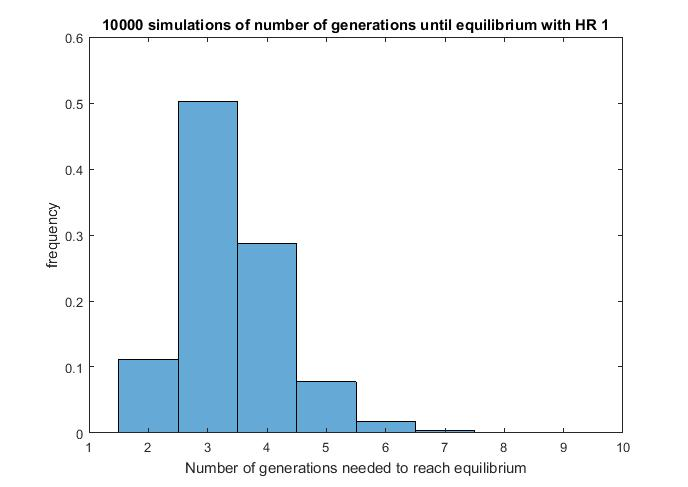
\includegraphics[width=\textwidth]{GenormHistogramAantalgen}
        \caption{10000 simulations of number of generations until equilibrium with HR 1/3}
        \label{fig:tiger}
    \end{subfigure}
    ~ %add desired spacing between images, e. g. ~, \quad, \qquad, \hfill etc. 
    %(or a blank line to force the subfigure onto a new line)
    \begin{subfigure}{0.4\textwidth}
        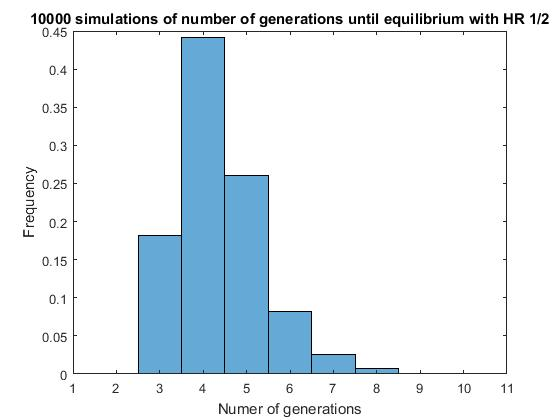
\includegraphics[width=\textwidth]{GenormHistogramAantalgen2}
        \caption{10000 simulations of number of generations until equilibrium with HR 1/2}
        \label{minimal happiness 1}
    \end{subfigure}
    \begin{subfigure}{0.4\textwidth}
        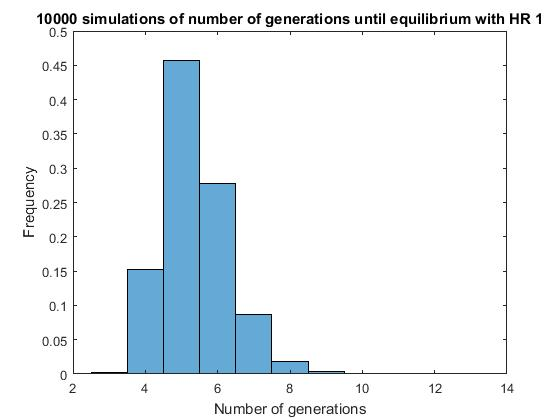
\includegraphics[width=\textwidth]{GenormHistogramAantalgen1}
        \caption{10000 simulations of number of generations until equilibrium with HR 1}
        \label{minimal happiness 2}
    \end{subfigure}
    \caption{The probability distribution of $Y$ (the number of generations until reaching the equilibrium) is approximated with a histogram of bin size 1. For each HR(1/4, 1/3, 1/2 and 1), 10000 simulations were ran.}\label{fig:histogram}
\end{figure}

From figure \ref{fig:histogram}, we see the distribution of $Y$ is quite similar to the binomial distribution. But we don't think that it is binomially distributed because more simulation does not give a more symmetrical distribution. It is not clear for us yet how it is distributed.\\
\\
Interesting to note though, is that both the mean and the variance increase with the happiness rule. In line with the following section, we see a relatively small mean and relatively often large number of generations.\\
\textbf{Partial explanation.} While not immediately intuitive, the relatively small mean cannot be immediately explained. However we do have an explanation for the relatively high frequency for the large number of generations. If, after a few generations, we do not have equilibrium, moving to a better location gets harder (see next section for precise details). Thus, reaching equilibrium eats relatively much time.